% =================================================================================================
% apresentacao.tex — Defesa de TCC (Beamer)
% "Ferramenta Baseada em DSL para o Apoio ao Ensino de Autômatos Finitos com Simulação Visual"
% João Thomaz Vieira e Klaus Siegfried Beckmann — Orientador: Prof. Diógenes Cogo Furlan — UTP 2026
%
% Compilar: pdflatex apresentacao.tex  (2x, para o índice/roteiro)
%
% ROTEIRO DE TEMPO (~35 min, faixa alvo 30–40):
%   1. Introdução .................. ~5 min
%   2. Fundamentação Teórica ....... ~8 min
%   3. Trabalhos Relacionados ...... ~4 min
%   4. Projeto da DSL (Autosim) .... ~5 min
%   5. Implementação ............... ~8 min
%   6. Demonstração e Resultados ... ~6 min
%   7. Conclusão ................... ~3 min
%   (+ arguição/perguntas da banca)
% =================================================================================================

\documentclass[aspectratio=169,11pt]{beamer}

\usepackage[utf8]{inputenc}
\usepackage[T1]{fontenc}
\usepackage[brazilian]{babel}
\usepackage{lmodern}
\usepackage{amsmath,amssymb}
\usepackage{listings}
\usepackage{booktabs}
\usepackage{colortbl}
\usepackage{tikz}
\usetikzlibrary{arrows.meta,positioning}
\usepackage{graphicx}

% ----- Tema -----------------------------------------------------------------------------------
\usetheme{Madrid}
\usecolortheme{whale}
\setbeamertemplate{navigation symbols}{}
\setbeamertemplate{caption}{\raggedright\insertcaption\par}
\setbeamercovered{transparent}

\definecolor{acento}{RGB}{0,90,156}
\setbeamercolor{structure}{fg=acento}
\setbeamercolor{block title}{bg=acento,fg=white}
\setbeamercolor{block body}{bg=acento!8}

% Slide de abertura de cada seção com o roteiro destacado
\AtBeginSection[]{%
  \begin{frame}{Roteiro}
    \tableofcontents[currentsection]
  \end{frame}%
}

% ----- Estilo de código: DSL Autosim (.asl) ---------------------------------------------------
\lstdefinelanguage{asl}{
  morekeywords={alfabeto,automato,AFD,AFN,estados,inicial,finais,transicoes,simular,com,epsilon,eps},
  sensitive=false,
  morecomment=[l]{//},
  morestring=[b]",
  morestring=[b]',
}
\lstset{
  basicstyle=\ttfamily\footnotesize,
  keywordstyle=\color{acento}\bfseries,
  commentstyle=\color{gray}\itshape,
  stringstyle=\color{orange!80!black},
  showstringspaces=false,
  columns=fullflexible,
  keepspaces=true,
  frame=single,
  framesep=4pt,
  rulecolor=\color{gray!40},
  aboveskip=4pt,belowskip=2pt,
}

% ----- Metadados ------------------------------------------------------------------------------
\title[Autosim: DSL para Ensino de Autômatos]{Ferramenta Baseada em Linguagem de Domínio Específico para o Apoio ao Ensino de Autômatos Finitos com Simulação Visual Interativa}
\author[Vieira \and Beckmann]{João Thomaz Vieira \and Klaus Siegfried Beckmann}
\institute[UTP]{Bacharelado em Ciência da Computação\\Universidade Tuiuti do Paraná\\[2pt]\footnotesize Orientador: Prof. Diógenes Cogo Furlan}
\date{Curitiba, 2026}

\begin{document}

% =================================================================================================
{\setbeamertemplate{footline}{}
\begin{frame}[plain]
  \titlepage
\end{frame}}

\begin{frame}{Roteiro}
  \tableofcontents
\end{frame}

% =================================================================================================
\section{Introdução}

\begin{frame}{Contexto e motivação}
  \begin{itemize}
    \item O estudo de \textbf{autômatos finitos e linguagens formais} é um dos pilares da
          formação em Ciência da Computação (máquinas abstratas, limites da computação, compiladores).
    \item Apesar da importância, é uma disciplina \textbf{reconhecidamente desafiadora}.
    \item Segundo Morazán e Antunez (2014), a dificuldade vem de uma causa precisa:
      \begin{quote}
        o estudante projeta autômatos e prova sua correção \textbf{sem poder experimentar} nem
        obter \textbf{retroalimentação imediata}, ao contrário do que ocorre na programação.
      \end{quote}
    \item Há um distanciamento entre o \textbf{formalismo simbólico} e a \textbf{prática computacional}.
  \end{itemize}
\end{frame}

\begin{frame}{O problema: as ferramentas existentes}
  Ferramentas de apoio (como o \textbf{JFLAP}) adotam uma abordagem \textbf{exclusivamente visual}
  (arrastar e soltar). Isso traz limitações relevantes:
  \begin{itemize}
    \item A descrição do autômato \textbf{não é textual} $\rightarrow$ dificulta versionamento
          (Git) e compartilhamento.
    \item \textbf{Não há validação formal} da estrutura com mensagens de erro claras e localizadas.
    \item O estudante que erra na construção \textbf{não recebe um diagnóstico preciso} do problema.
  \end{itemize}
  \vspace{4pt}
  \begin{block}{Lacuna}
    Falta uma ferramenta que una o \textbf{rigor da descrição textual} ao \textbf{diagnóstico de um
    compilador} e à \textbf{interatividade da simulação visual}.
  \end{block}
\end{frame}

\begin{frame}{A proposta: Autosim}
  Uma ferramenta educacional que acopla diretamente:
  \begin{columns}[T]
    \begin{column}{0.5\textwidth}
      \begin{block}{DSL textual}
        Linguagem de domínio específico, declarativa e em português, para descrever AFDs e AFNs.
      \end{block}
      \begin{block}{Compilador pedagógico}
        Análises léxica, sintática e semântica, com \textbf{diagnósticos localizados} (linha e coluna).
      \end{block}
    \end{column}
    \begin{column}{0.5\textwidth}
      \begin{block}{Interface gráfica interativa}
        Renderiza o diagrama a partir do texto e \textbf{anima a simulação passo a passo}.
      \end{block}
      \begin{alertblock}{Contribuição central}
        Acoplamento direto entre a descrição textual e a geração automática de uma interface
        gráfica sincronizada.
      \end{alertblock}
    \end{column}
  \end{columns}
\end{frame}

\begin{frame}{Objetivos}
  \textbf{Objetivo geral:} desenvolver uma ferramenta educacional que integra a descrição textual
  de autômatos, sua compilação pedagógica e sua simulação visual em um único ambiente.
  \vspace{6pt}
  \begin{block}{Objetivos específicos}
    \begin{enumerate}
      \item Projetar uma \textbf{DSL} textual para descrever AFDs e AFNs (gramática em EBNF);
      \item Implementar um \textbf{compilador pedagógico} (léxico, sintático e semântico) com
            diagnósticos localizados;
      \item Desenvolver um \textbf{simulador} de cadeias sobre os autômatos descritos;
      \item Construir uma \textbf{interface gráfica} que renderize o diagrama e anime a simulação;
      \item \textbf{Validar} a ferramenta com autômatos clássicos e cenários de erro induzido.
    \end{enumerate}
  \end{block}
\end{frame}

% =================================================================================================
\section{Fundamentação Teórica}

\begin{frame}{Autômatos finitos}
  \begin{columns}[T]
    \begin{column}{0.58\textwidth}
      Um \textbf{AFD} é uma quíntupla $M = (Q, \Sigma, \delta, q_0, F)$:
      \begin{itemize}
        \item $Q$ — conjunto finito de estados;
        \item $\Sigma$ — alfabeto de entrada;
        \item $\delta: Q \times \Sigma \to Q$ — função de transição;
        \item $q_0 \in Q$ — estado inicial;
        \item $F \subseteq Q$ — estados de aceitação.
      \end{itemize}
      \vspace{4pt}
      No \textbf{AFN}, a transição leva a um \emph{conjunto} de estados
      ($\delta: Q \times (\Sigma \cup \{\varepsilon\}) \to 2^{Q}$), admitindo
      transições vazias~$\varepsilon$.
    \end{column}
    \begin{column}{0.42\textwidth}
      \begin{block}{Linguagem reconhecida}
        \[ L(M) = \{\, w \in \Sigma^* \mid \hat\delta(q_0, w) \in F \,\} \]
      \end{block}
      AFD e AFN são \textbf{equivalentes} em poder de reconhecimento
      (construção de subconjuntos) e definem exatamente as
      \textbf{linguagens regulares}.
    \end{column}
  \end{columns}
\end{frame}

\begin{frame}{Gramáticas e a Hierarquia de Chomsky}
  Restrições sobre a forma das regras definem classes de linguagens:
  \vspace{4pt}
  \begin{center}
    \small
    \begin{tabular}{@{}clll@{}}
      \toprule
      \textbf{Tipo} & \textbf{Classe} & \textbf{Forma das regras} & \textbf{Modelo} \\
      \midrule
      0 & Recursiv.\ enumeráveis & $\alpha \to \beta$ & Máquina de Turing \\
      1 & Sensíveis ao contexto & $\alpha A \beta \to \alpha \gamma \beta$ & Autômato lin.\ limitado \\
      2 & Livres de contexto & $A \to \gamma$ & Autômato com pilha \\
      \rowcolor{acento!12}
      3 & \textbf{Regulares} & $A \to aB \mid A \to a$ & \textbf{Autômato finito} \\
      \bottomrule
    \end{tabular}
  \end{center}
  \vspace{4pt}
  As \textbf{gramáticas regulares (Tipo 3)} geram exatamente a classe reconhecida pelos
  \textbf{autômatos finitos} — o formalismo central deste trabalho.
\end{frame}

\begin{frame}{Compiladores: as fases de análise}
  Um compilador traduz um programa-fonte verificando sua consistência em fases sucessivas:
  \vspace{6pt}
  \begin{center}
    \begin{tikzpicture}[
        node distance=6mm and 8mm,
        etapa/.style={draw=acento,fill=acento!10,rounded corners,align=center,
                      minimum height=10mm,inner sep=4pt,font=\footnotesize},
        seta/.style={-{Stealth[length=2mm]},thick,acento}]
      \node[etapa] (a) {Análise\\\textbf{Léxica}};
      \node[etapa,right=of a] (b) {Análise\\\textbf{Sintática}};
      \node[etapa,right=of b] (c) {Análise\\\textbf{Semântica}};
      \draw[seta] (a)--(b); \draw[seta] (b)--(c);
      \node[below=1mm of a,font=\scriptsize\itshape,text width=24mm,align=center] {texto $\to$ \emph{tokens}};
      \node[below=1mm of b,font=\scriptsize\itshape,text width=24mm,align=center] {\emph{tokens} $\to$ AST};
      \node[below=1mm of c,font=\scriptsize\itshape,text width=26mm,align=center] {consistência de significado};
    \end{tikzpicture}
  \end{center}
  \vspace{2pt}
  \begin{itemize}
    \item \textbf{Léxica:} agrupa caracteres em unidades léxicas (\emph{tokens}) — via expressões regulares.
    \item \textbf{Sintática:} organiza os \emph{tokens} em uma \textbf{Árvore Sintática Abstrata (AST)}.
    \item \textbf{Semântica:} verifica regras que a gramática não captura (referências, consistência).
  \end{itemize}
\end{frame}

\begin{frame}{Linguagens de Domínio Específico (DSL)}
  \begin{block}{Definição (Fowler, 2010)}
    Uma DSL é ``uma linguagem de programação de \textbf{expressividade limitada}, voltada para um
    \textbf{domínio específico}''.
  \end{block}
  \begin{itemize}
    \item Ganha \textbf{concisão e legibilidade} no seu domínio, ao custo da generalidade.
    \item \textbf{DSL interna:} embutida em uma linguagem hospedeira.
    \item \textbf{DSL externa:} sintaxe própria, exige um \textbf{compilador dedicado}.
  \end{itemize}
  \vspace{4pt}
  \begin{center}
    \emph{A Autosim é uma \textbf{DSL externa}} — com sintaxe própria e um compilador implementado em Rust.
  \end{center}
\end{frame}

\begin{frame}{Por que Rust?}
  \begin{itemize}
    \item Linguagem de sistemas com \textbf{desempenho de C/C++} e \textbf{segurança de memória}
          verificada em tempo de compilação (\emph{ownership} e \emph{borrowing}, sem coletor de lixo).
    \item \textbf{Segurança de tipos} facilita representar \emph{tokens}, nós de AST e estados de
          autômatos sem inconsistências em tempo de execução.
    \item Estilo \textbf{funcional} (\emph{traits}, iteradores) favorece compor as fases de análise
          de forma clara e modular.
    \item Ecossistema maduro (\textbf{Cargo}) com bibliotecas para \emph{lexing}, \emph{parsing} e GUI.
  \end{itemize}
\end{frame}

% =================================================================================================
\section{Trabalhos Relacionados}

\begin{frame}{Panorama das ferramentas existentes}
  \begin{itemize}
    \item \textbf{JFLAP} — referência mundial; gráfica (arrastar e soltar); cobre toda a hierarquia
          de Chomsky. \emph{Sem} representação textual, versionamento ou diagnóstico.
    \item \textbf{GAM} (UFLA) — autômatos finitos e expressões regulares; \emph{desktop} (C++/GTK);
          limitado a 10 estados e 3 símbolos.
    \item \textbf{Simulador UFSC} — aplicação \emph{web} (AFD/AFN, pilha e Turing); elimina barreiras
          de instalação, mas mantém a construção puramente gráfica.
    \item \textbf{AutomatoGraph} — foco em AFDs; \textbf{gera a gramática regular} correspondente;
          simulação apenas parcialmente visual.
    \item \textbf{Análise Léxica em Rust} (Bruzzone, 2023) — rigor de engenharia (lexer via autômatos),
          mas \emph{sem} suporte educacional / interface para iniciantes.
  \end{itemize}
\end{frame}

\begin{frame}{Análise comparativa}
  \begin{center}
    \scriptsize
    \setlength{\tabcolsep}{4pt}
    \begin{tabular}{@{}lccccc@{}}
      \toprule
      \textbf{Trabalho} & \textbf{DSL} & \textbf{Versiona-} & \textbf{Compilador/} & \textbf{Simulação} & \textbf{Voltada} \\
                        & \textbf{textual} & \textbf{mento} & \textbf{diagnóstico} & \textbf{visual} & \textbf{ao ensino} \\
      \midrule
      Análise Léxica em Rust & Não & Sim & Não & Não & Não \\
      JFLAP                  & Não & Não & Não & Sim & Sim \\
      GAM                    & Não & Não & Não & Sim & Sim \\
      Simulador UFSC         & Não & Não & Não & Sim & Sim \\
      AutomatoGraph          & Não & Não & Não & Parcial & Sim \\
      \rowcolor{acento!15}
      \textbf{Autosim (este trabalho)} & \textbf{Sim} & \textbf{Sim} & \textbf{Sim} & \textbf{Sim} & \textbf{Sim} \\
      \bottomrule
    \end{tabular}
  \end{center}
  \vspace{6pt}
  \begin{center}
    Nenhuma ferramenta une \textbf{descrição textual + compilador com diagnóstico + simulação visual}.\\
    \textbf{É essa lacuna que a Autosim ocupa.}
  \end{center}
\end{frame}

% =================================================================================================
\section{Projeto da DSL (Autosim)}

\begin{frame}[fragile]{A linguagem: um exemplo}
  DSL externa, sintaxe em \textbf{português}; cada arquivo \texttt{.asl} tem um alfabeto comum
  e um ou mais autômatos, seguidos de comandos de simulação.
  \begin{lstlisting}[language=asl]
alfabeto { 'a', 'b' }

automato AFD exemplo_afd {
    estados { q0, q1, q2 }
    inicial q0
    finais { q2 }
    transicoes {
        q0 -> q1 com 'a'      q1 -> q2 com 'b'
        q0 -> q0 com 'b'      q1 -> q1 com 'a'
        q2 -> q2 com 'a'      q2 -> q2 com 'b'
    }
}

simular exemplo_afd com "ab"      // aceita
simular exemplo_afd com "bbb"     // rejeita
  \end{lstlisting}
\end{frame}

\begin{frame}[fragile]{Gramática formal (EBNF)}
  Linguagem \textbf{livre de contexto}, analisável por \emph{parser} descendente preditivo com um
  símbolo de \emph{lookahead}:
  \begin{lstlisting}[basicstyle=\ttfamily\scriptsize]
programa            ::= declaracao_alfabeto item*
declaracao_alfabeto ::= "alfabeto" "{" char_literal ("," char_literal)* [","] "}"
item                ::= declaracao_automato | comando_simulacao
declaracao_automato ::= "automato" tipo_automato ident "{"
                            "estados" "{" ident ("," ident)* [","] "}"
                            "inicial" ident
                            "finais"  "{" ident ("," ident)* [","] "}"
                            "transicoes" "{" transicao* "}" "}"
tipo_automato       ::= "AFD" | "AFN"
transicao           ::= ident "->" ident "com" (char_literal | "epsilon" | "eps")
comando_simulacao   ::= "simular" ident "com" cadeia_literal
  \end{lstlisting}
  \footnotesize 11 palavras reservadas, \emph{case-insensitive}.
\end{frame}

\begin{frame}{Decisões de projeto}
  \begin{itemize}
    \item \textbf{Declaração única de alfabeto} — reforça o conceito teórico e simplifica a
          verificação semântica (um único conjunto de referência).
    \item \textbf{Classificação explícita AFD/AFN} — permite verificações específicas por tipo
          (ex.: determinismo só para AFD).
    \item \textbf{Case-insensitive} — \texttt{AFD}, \texttt{afd}, \texttt{Afd} são equivalentes;
          reduz a carga cognitiva do estudante.
    \item \textbf{Suporte a transições $\varepsilon$} — palavras-chave \texttt{epsilon} / \texttt{eps}
          para AFNs com movimentos vazios.
  \end{itemize}
\end{frame}

% =================================================================================================
\section{Implementação}

\begin{frame}{Pipeline de compilação}
  \begin{center}
    \begin{tikzpicture}[
        node distance=5mm,
        etapa/.style={draw=acento,fill=acento!10,rounded corners,align=center,
                      minimum height=12mm,text width=20mm,inner sep=3pt,font=\scriptsize},
        seta/.style={-{Stealth[length=2mm]},thick,acento}]
      \node[etapa] (f) {Arquivo\\\texttt{.asl}};
      \node[etapa,right=of f] (l) {Analisador\\Léxico\\\textbf{(Logos)}};
      \node[etapa,right=of l] (p) {Analisador\\Sintático\\\textbf{(Chumsky)}};
      \node[etapa,right=of p] (s) {Analisador\\Semântico};
      \node[etapa,right=of s] (r) {Simulador};
      \node[etapa,right=of r] (g) {Interface\\Gráfica\\\textbf{(Iced)}};
      \draw[seta](f)--(l);\draw[seta](l)--(p);\draw[seta](p)--(s);\draw[seta](s)--(r);\draw[seta](r)--(g);
    \end{tikzpicture}
  \end{center}
  \vspace{4pt}
  \begin{itemize}
    \item Fases executadas \textbf{sequencialmente}; em caso de erro, os diagnósticos são exibidos
          (via \textbf{Ariadne}) e a execução é interrompida antes da fase seguinte.
    \item Implementação em \textbf{Rust}, reaproveitando bibliotecas maduras do ecossistema.
  \end{itemize}
\end{frame}

\begin{frame}{Análise léxica e sintática}
  \begin{columns}[T]
    \begin{column}{0.5\textwidth}
      \begin{block}{Léxica — Logos}
        \begin{itemize}\footnotesize
          \item \emph{Lexer} gerado a partir de anotações no tipo \texttt{Token}.
          \item Gera um AFD para reconhecimento eficiente dos padrões.
          \item Palavras reservadas \emph{case-insensitive}; espaços e comentários (\texttt{//}) descartados.
          \item Erro léxico $\to$ posição (linha/coluna) do caractere inválido.
        \end{itemize}
      \end{block}
    \end{column}
    \begin{column}{0.5\textwidth}
      \begin{block}{Sintática — Chumsky}
        \begin{itemize}\footnotesize
          \item \emph{Parser combinators}: a gramática é codificada compondo funções.
          \item Produz a \textbf{AST}, eliminando ruídos sintáticos (delimitadores).
          \item \emph{Spans} referenciam índices de \emph{token} para localizar erros.
        \end{itemize}
      \end{block}
    \end{column}
  \end{columns}
\end{frame}

\begin{frame}{Análise semântica — 3 fases estáticas}
  \begin{enumerate}
    \item \textbf{Tabela de símbolos:} detecta símbolo/estado/autômato \textbf{duplicado}.
    \item \textbf{Verificação de referências:} estado inicial/final/origem/destino não declarado;
          símbolo fora do alfabeto; simulação de autômato inexistente.
    \item \textbf{Verificação de determinismo} (só para AFD):
          \begin{itemize}
            \item ausência de transições $\varepsilon$;
            \item unicidade de transição por par (estado, símbolo).
          \end{itemize}
  \end{enumerate}
  \vspace{2pt}
  \begin{block}{}
    Os erros são \textbf{acumulados} e apresentados em conjunto — o estudante vê todos os problemas
    de uma só vez.
  \end{block}
\end{frame}

\begin{frame}{Simulador}
  \begin{itemize}
    \item Executa a função de transição sobre a cadeia, registrando \textbf{todas as configurações
          intermediárias}.
    \item \textbf{Representação unificada} por conjuntos de estados (\texttt{BTreeSet}):
          \begin{itemize}
            \item AFD $\to$ conjunto com exatamente um estado;
            \item AFN $\to$ conjunto com múltiplos estados (busca em largura, com fecho-$\varepsilon$).
          \end{itemize}
    \item Guarda o \textbf{histórico completo} $\Rightarrow$ navegação \textbf{bidirecional}
          (avançar / retroceder) durante a execução.
  \end{itemize}
\end{frame}

\begin{frame}{Interface gráfica (Iced)}
  \begin{itemize}
    \item \textbf{Renderização automática} do diagrama de estados a partir do texto-fonte.
    \item \textbf{Simulação passo a passo}, com reprodução automática (800 ms/passo):
          destaca o estado corrente, a transição percorrida e a cadeia consumida.
    \item \textbf{Navegação} do diagrama: \emph{pan} (arrastar) e \emph{zoom} (rolar), com botão
          \textbf{Centralizar}.
    \item Painel muda de cor conforme o \textbf{veredito}: \textcolor{green!50!black}{\textbf{verde
          (aceita)}} / \textcolor{red!70!black}{\textbf{vermelho (rejeita)}}.
  \end{itemize}
\end{frame}

\begin{frame}{Diagnóstico de erros (Ariadne)}
  \begin{itemize}
    \item Toda mensagem inclui \textbf{linha e coluna}, um \textbf{trecho do código com realce
          colorido} e uma \textbf{seta} apontando para o ponto do erro.
    \item Descrição do problema \textbf{em português}.
  \end{itemize}
  \vspace{4pt}
  \begin{exampleblock}{Exemplos}
    \begin{itemize}
      \item Caractere \texttt{\%} não reconhecido $\to$ \emph{``token inválido''}.
      \item AFD com transição $\varepsilon$ $\to$ \emph{``AFD não pode ter epsilon''}.
      \item Falta a palavra \texttt{inicial} $\to$ \emph{``esperava 'inicial'\,''}.
    \end{itemize}
  \end{exampleblock}
  \begin{center}
    Substitui o ``tentar e errar visual'' por \textbf{retroalimentação imediata e precisa}.
  \end{center}
\end{frame}

% =================================================================================================
\section{Demonstração e Resultados}

\begin{frame}{Interface — visão geral}
  \begin{center}
    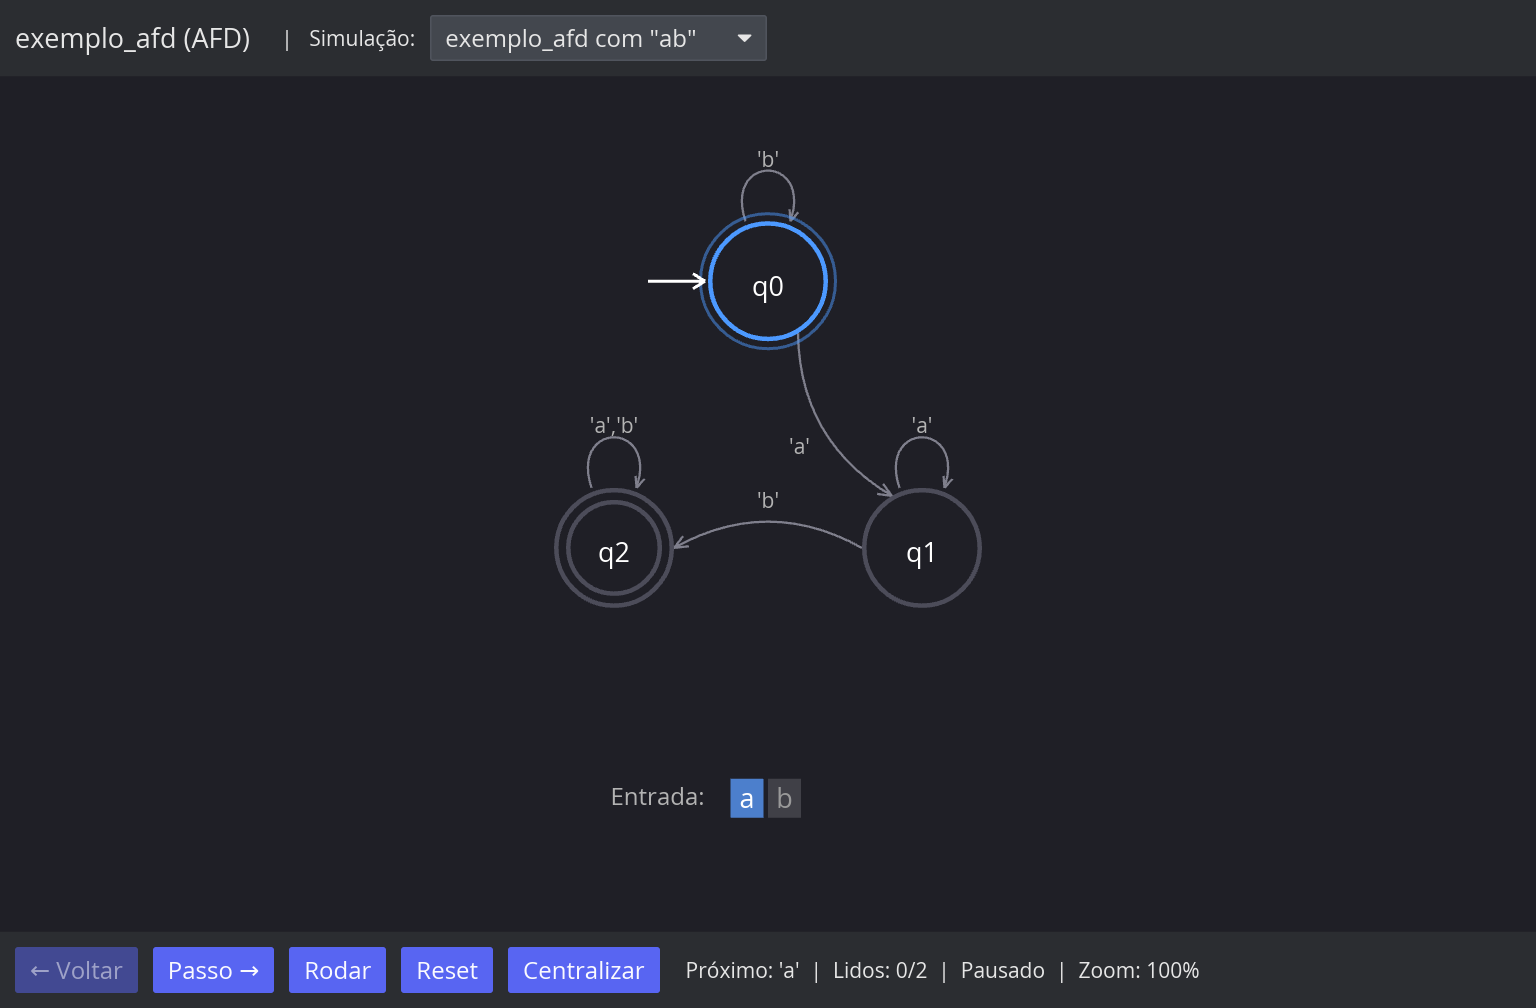
\includegraphics[height=0.82\textheight]{img/interface_visao_geral.png}
  \end{center}
\end{frame}

\begin{frame}{Simulação — veredito de \textcolor{green!50!black}{aceitação}}
  \begin{center}
    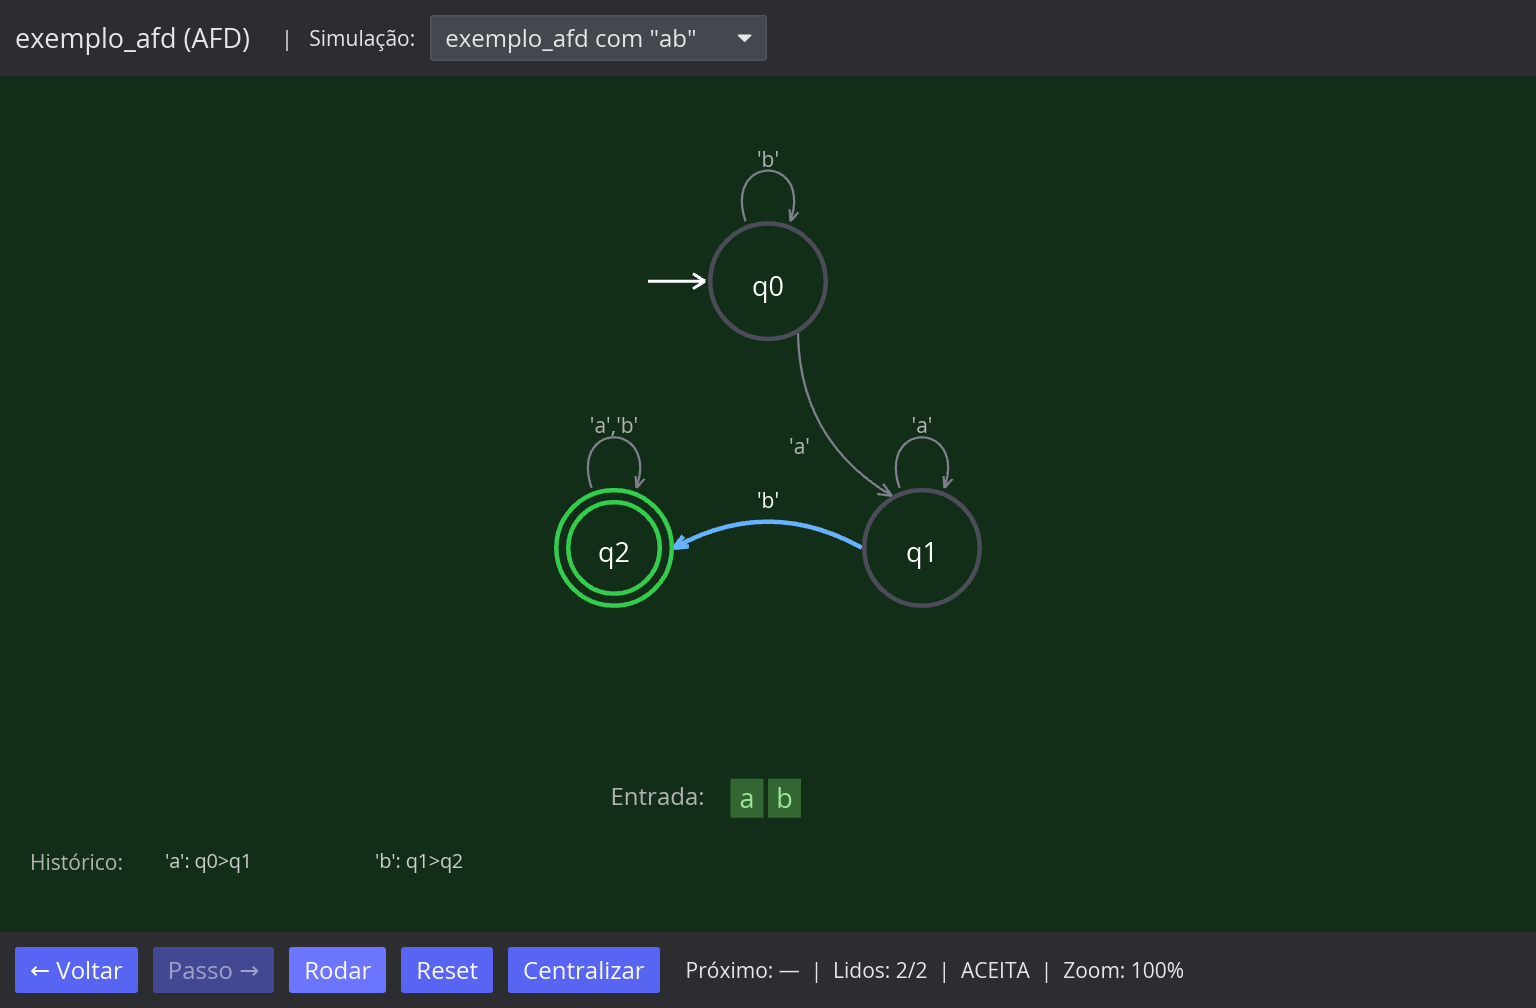
\includegraphics[height=0.82\textheight]{img/interface_simulacao_aceita.png}
  \end{center}
\end{frame}

\begin{frame}{Simulação — veredito de \textcolor{red!70!black}{rejeição}}
  \begin{center}
    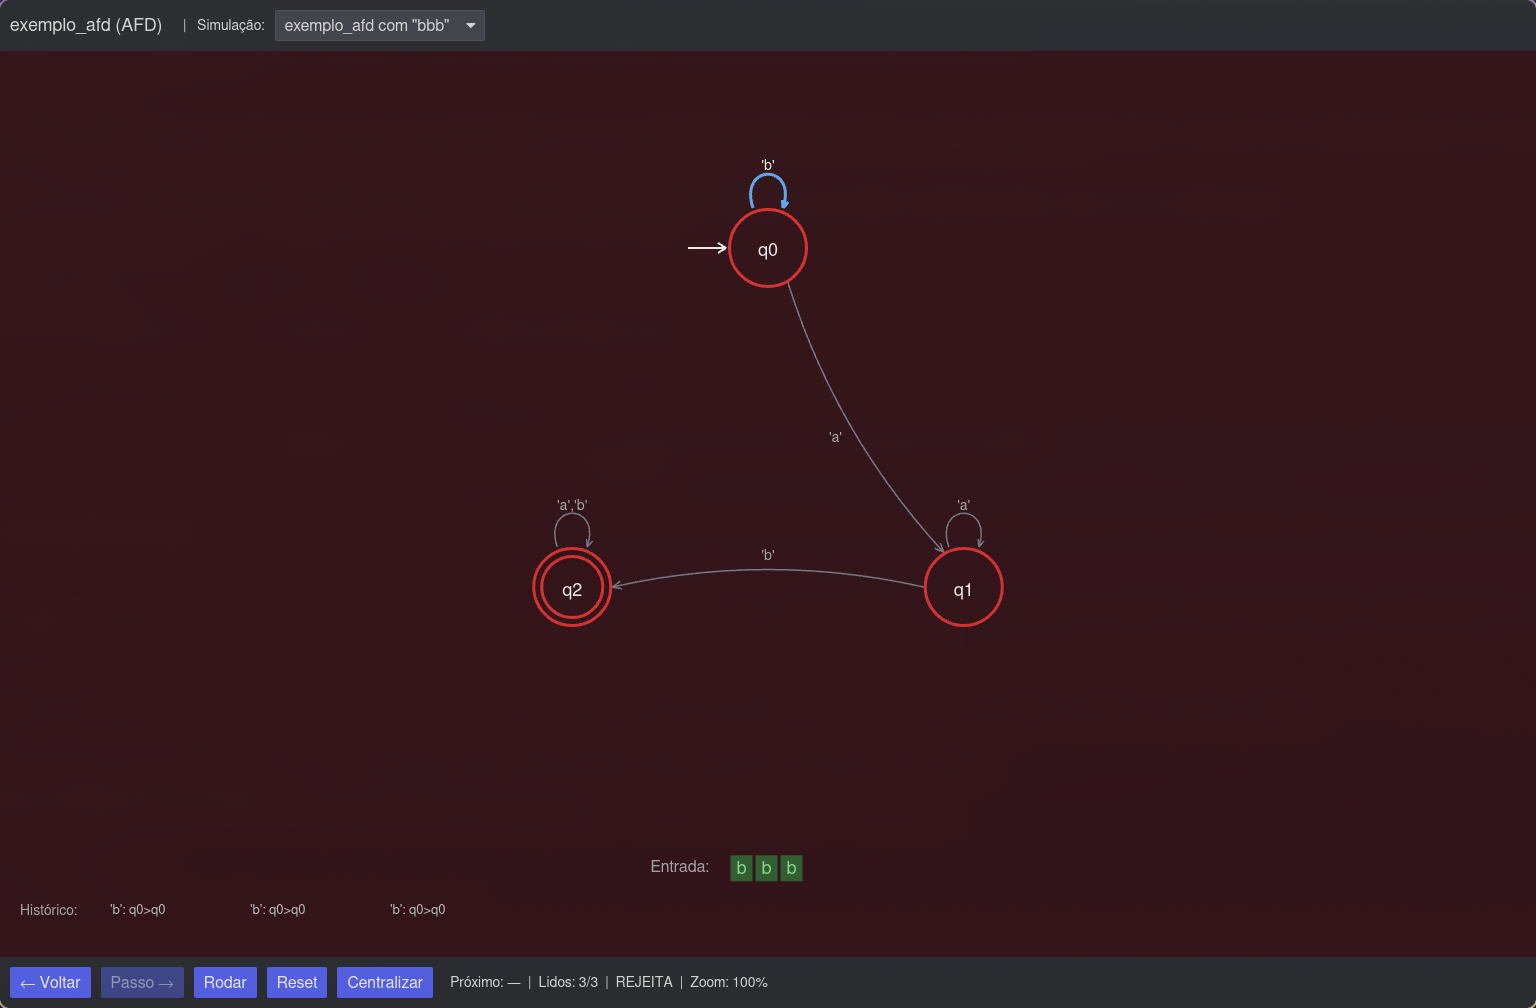
\includegraphics[height=0.82\textheight]{img/interface_simulacao_rejeita.png}
  \end{center}
\end{frame}

\begin{frame}{AFN-$\varepsilon$ e navegação em diagramas grandes}
  \begin{columns}[c]
    \begin{column}{0.5\textwidth}
      \centering
      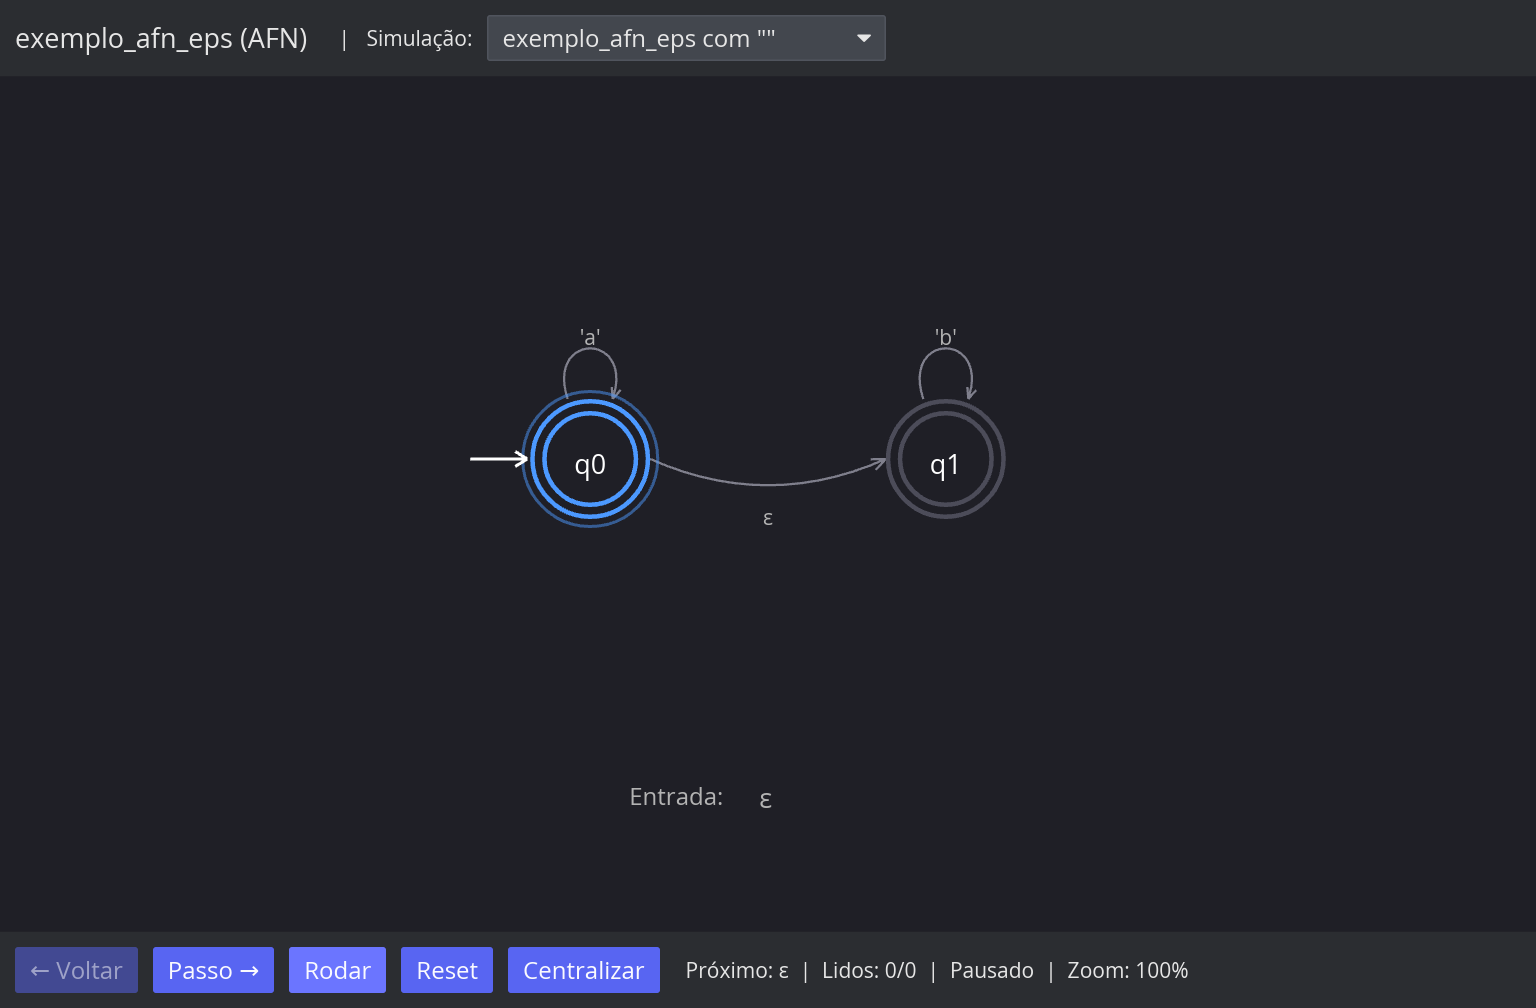
\includegraphics[width=\textwidth]{img/interface_afn_epsilon.png}\\
      {\scriptsize AFN com transições $\varepsilon$}
    \end{column}
    \begin{column}{0.5\textwidth}
      \centering
      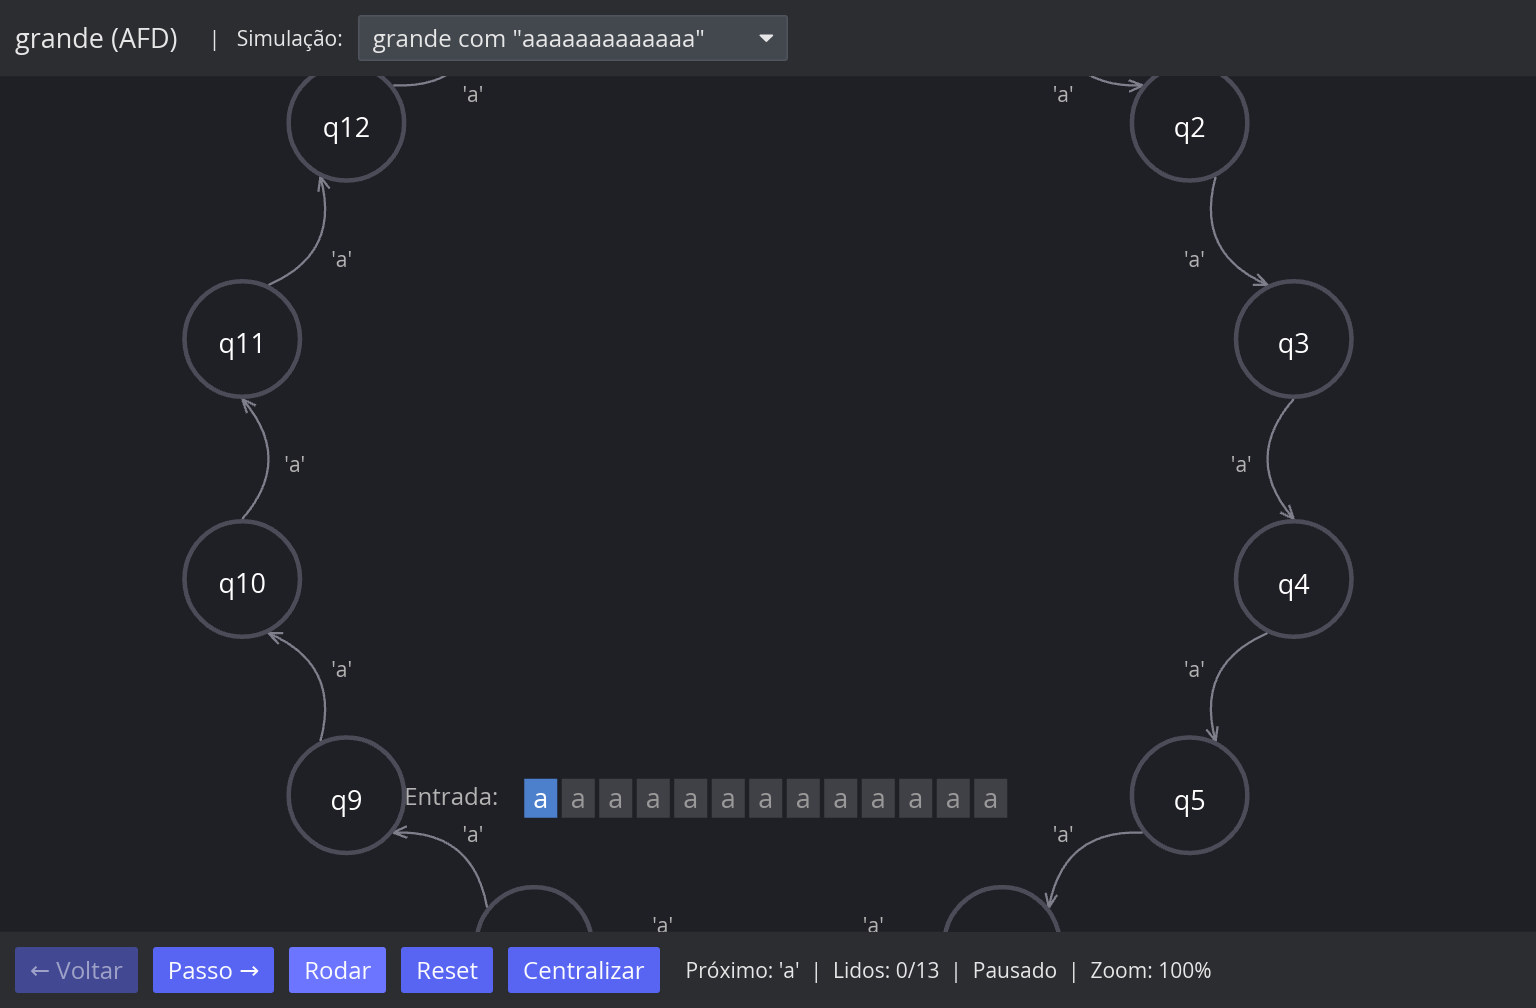
\includegraphics[width=\textwidth]{img/interface_automato_grande.png}\\
      {\scriptsize AFD de 14 estados — \emph{pan} e \emph{zoom}}
    \end{column}
  \end{columns}
\end{frame}

\begin{frame}{Validação — testes automatizados}
  \begin{columns}[c]
    \begin{column}{0.45\textwidth}
      \begin{block}{42 testes automatizados}
        \begin{tabular}{@{}lc@{}}
          Analisador léxico    & 12 \\
          Analisador sintático & 15 \\
          Analisador semântico & 15 \\
          \midrule
          \textbf{Total}       & \textbf{42} \\
        \end{tabular}
      \end{block}
    \end{column}
    \begin{column}{0.55\textwidth}
      \begin{itemize}
        \item Cobrem reconhecimento de \emph{tokens}, construção da AST e todas as verificações
              semânticas.
        \item \textbf{Todos os resultados} concordaram com o esperado.
      \end{itemize}
    \end{column}
  \end{columns}
\end{frame}

\begin{frame}{Validação — simulações com autômatos clássicos}
  Autômatos de Hopcroft (2006) e Sipser (2012):
  \begin{center}
    \scriptsize
    \begin{tabular}{@{}llcc@{}}
      \toprule
      \textbf{Autômato} & \textbf{Cadeia} & \textbf{Esperado} & \textbf{Obtido} \\
      \midrule
      AFD: contém 01 & \texttt{1101} & Aceita & Aceita \\
      AFD: contém 01 & \texttt{111}  & Rejeita & Rejeita \\
      AFN: termina em 01 & \texttt{001} & Aceita & Aceita \\
      AFN: termina em 01 & \texttt{010} & Rejeita & Rejeita \\
      AFN-$\varepsilon$: $a^*b^*$ & \texttt{aabb} & Aceita & Aceita \\
      AFN-$\varepsilon$: $a^*b^*$ & \texttt{ba} & Rejeita & Rejeita \\
      AFN-$\varepsilon$: $a^*b^*$ & $\varepsilon$ & Aceita & Aceita \\
      \bottomrule
    \end{tabular}
  \end{center}
  \begin{center}
    Todos os vereditos corretos $\Rightarrow$ \textbf{correção do simulador} (AFD e AFN-$\varepsilon$).
  \end{center}
\end{frame}

\begin{frame}{Validação — cenários de diagnóstico de erro}
  Arquivos com \textbf{erros propositais}, simulando o uso real por estudantes:
  \begin{center}
    \scriptsize
    \begin{tabular}{@{}lll@{}}
      \toprule
      \textbf{Arquivo} & \textbf{Tipo de erro} & \textbf{Diagnóstico} \\
      \midrule
      \texttt{sema\_error.asl} & 4 erros semânticos & 4 mensagens localizadas \\
      \texttt{sema\_dfa\_epsilon.asl} & AFD com $\varepsilon$ & ``AFD não pode ter epsilon'' \\
      \texttt{sema\_nondeterministic.asl} & AFD não-determinístico & Transição conflitante \\
      \texttt{parse\_error.asl} & Falta \texttt{inicial} & ``esperava 'inicial'\,'' \\
      \texttt{symbol\_error.asl} & Caractere inválido & ``token inválido'' \\
      \bottomrule
    \end{tabular}
  \end{center}
  \begin{center}
    Todas as mensagens com \textbf{linha, coluna, trecho realçado e descrição em português}.
  \end{center}
\end{frame}

% =================================================================================================
\section{Conclusão}

\begin{frame}{Contribuições}
  A \textbf{Autosim} preenche a lacuna entre a descrição formal textual e a visualização gráfica:
  \begin{itemize}
    \item Uma \textbf{DSL} declarativa em português para AFDs e AFNs (com $\varepsilon$),
          formalizada em EBNF.
    \item Um \textbf{compilador pedagógico completo} (Logos + Chumsky + análise semântica) com
          \textbf{diagnósticos localizados e coloridos}.
    \item Um \textbf{simulador} com histórico e navegação bidirecional.
    \item Uma \textbf{interface gráfica} que renderiza e anima a simulação passo a passo.
    \item Validação com \textbf{42 testes} e simulações clássicas — \textbf{todos corretos}.
  \end{itemize}
\end{frame}

\begin{frame}{Limitações e trabalhos futuros}
  \begin{columns}[T]
    \begin{column}{0.5\textwidth}
      \begin{block}{Limitações}
        \begin{itemize}\footnotesize
          \item Alfabeto único por arquivo.
          \item Sem modo puramente textual (CLI).
          \item Um arquivo por execução (sem módulos).
          \item Sem editor embutido com realce.
          \item Sem conversão AFN$\to$AFD / minimização.
        \end{itemize}
      \end{block}
    \end{column}
    \begin{column}{0.5\textwidth}
      \begin{block}{Trabalhos futuros}
        \begin{itemize}\footnotesize
          \item Editor com realce na própria interface.
          \item Alfabetos distintos por autômato.
          \item Conversão AFN$\to$AFD, minimização e extração de gramáticas.
          \item Modo CLI para automação.
          \item \textbf{Estudos controlados com estudantes} (impacto pedagógico).
        \end{itemize}
      \end{block}
    \end{column}
  \end{columns}
\end{frame}

% =================================================================================================
{\setbeamercolor{background canvas}{bg=acento}
\begin{frame}[plain]
  \centering
  \vfill
  {\color{white}\Huge \textbf{Obrigado!}}\\[10pt]
  {\color{white}\large Perguntas?}\\[24pt]
  {\color{white!85}\footnotesize João Thomaz Vieira \quad$\cdot$\quad Klaus Siegfried Beckmann}\\[2pt]
  {\color{white!85}\footnotesize Orientador: Prof. Diógenes Cogo Furlan \quad$\cdot$\quad UTP, 2026}
  \vfill
\end{frame}}

\end{document}
